\section{Experiments}

\subsection{Setup}
\noindent \textbf{Dataset and Metric.} 
All experiments are conducted on the COCO 2017~\cite{lin2014microsoft} dataset, using the \texttt{train2017} split for training and \texttt{val2017} for evaluation. We report the standard COCO metrics, including AP~(averaged over uniformly sampled IoU thresholds ranging from 0.50-0.95 with a step size of 0.05), AP$_{50}$, AP$_{75}$, as well as AP at different scales: AP$_S$, AP$_M$, AP$_L$.

\noindent \textbf{Implementation Details.}
Our experiments are based on the RT-DETR architecture~\cite{zhao2024detrs}, with additional architectural and training refinements from RT-DETRv2~\cite{lv2024rt}, D-FINE~\cite{peng2024d}, and DEIM~\cite{huang2025deim}. For fair comparison, the core hyperparameters remain consistent with those in the corresponding baselines. 
The DSI employs a pre-trained and frozen DINOv3-ViT-B model as the semantic teacher. All evaluations are conducted using the COCO AP metrics, and inference latency (in milliseconds) is measured on a single NVIDIA T4 GPU under TensorRT FP16 precision.


\subsection{Comparison with SOTA}
We compare our proposed {RT-DETRv4} with recent state-of-the-art real-time detectors, including the latest YOLO series (YOLOv10~\cite{wang2024yolov10}, YOLOv11~\cite{yolo11}, YOLOv12~\cite{tian2025yolov12}, and YOLOv13~\cite{lei2025yolov13}) and DETR-based detectors (RT-DETR~\cite{zhao2024detrs}, RT-DETRv2~\cite{lv2024rt}, RT-DETRv3~\cite{wang2025rt}, D-FINE~\cite{peng2024d}, DEIM~\cite{huang2025deim}, and DEIMv2~\cite{huang2025real}). The results are illustrated in Figure~\ref{fig:coco_ap_latency}, and detailed statistics are provided in Table~\ref{tab:comparison}.
The results demonstrate that {RT-DETRv4} consistently achieves the best performance across all model scales (S, M, L, and X) without introducing any extra inference and deployment overhead.

Specifically, our \textbf{RT-DETRv4-L} achieves \textbf{55.4 AP} on COCO at \textbf{124 FPS}, outperforming YOLOv13-L (53.4 AP) and DEIM-L (54.7 AP) under comparable or even lower computational budgets.
The largest variant, \textbf{RT-DETRv4-X}, reaches \textbf{57.0 AP}, exceeding DEIM-X (56.5 AP) without introducing any inference overhead.
At smaller scales, \textbf{RT-DETRv4-S} and \textbf{RT-DETRv4-M} obtain \textbf{49.7} and \textbf{53.5 AP}, respectively, both clearly surpassing their DEIM counterparts (49.0 and 52.7 AP). 

To ensure a fair comparison within a similar latency regime, we report DEIMv2~\cite{huang2025real} results only in Figure~\ref{fig:coco_ap_latency} and exclude them from Table~\ref{tab:comparison}, as their models generally exhibit higher inference latency. 
Under comparable inference speeds, our RT-DETRv4-M surpasses DEIMv2-S by a large margin (53.5 AP vs. 50.9 AP at 169 FPS vs. 173 FPS), and RT-DETRv4-L further outperforms DEIMv2-M (55.4 AP vs. 53.0 AP at 124 FPS vs. 113 FPS).
These results fully demonstrate the effectiveness and great potential of the proposed method.
Although DEIMv2-X achieves stronger performance, its latency is also higher than that of RT-DETRv4-X.
Moreover, directly adopting DINOv3 as the backbone to obtain semantic richness is fundamentally constrained by model size and deployment cost, limiting it to the Tiny or Small variants of DINOv3 and making it difficult to scale to more powerful large-scale models. In contrast, our framework remains agnostic to both VFM type and scale, introducing no inference or deployment overhead, offering a more flexible and deployment-friendly solution.

\begin{figure*}[t]
    \centering
    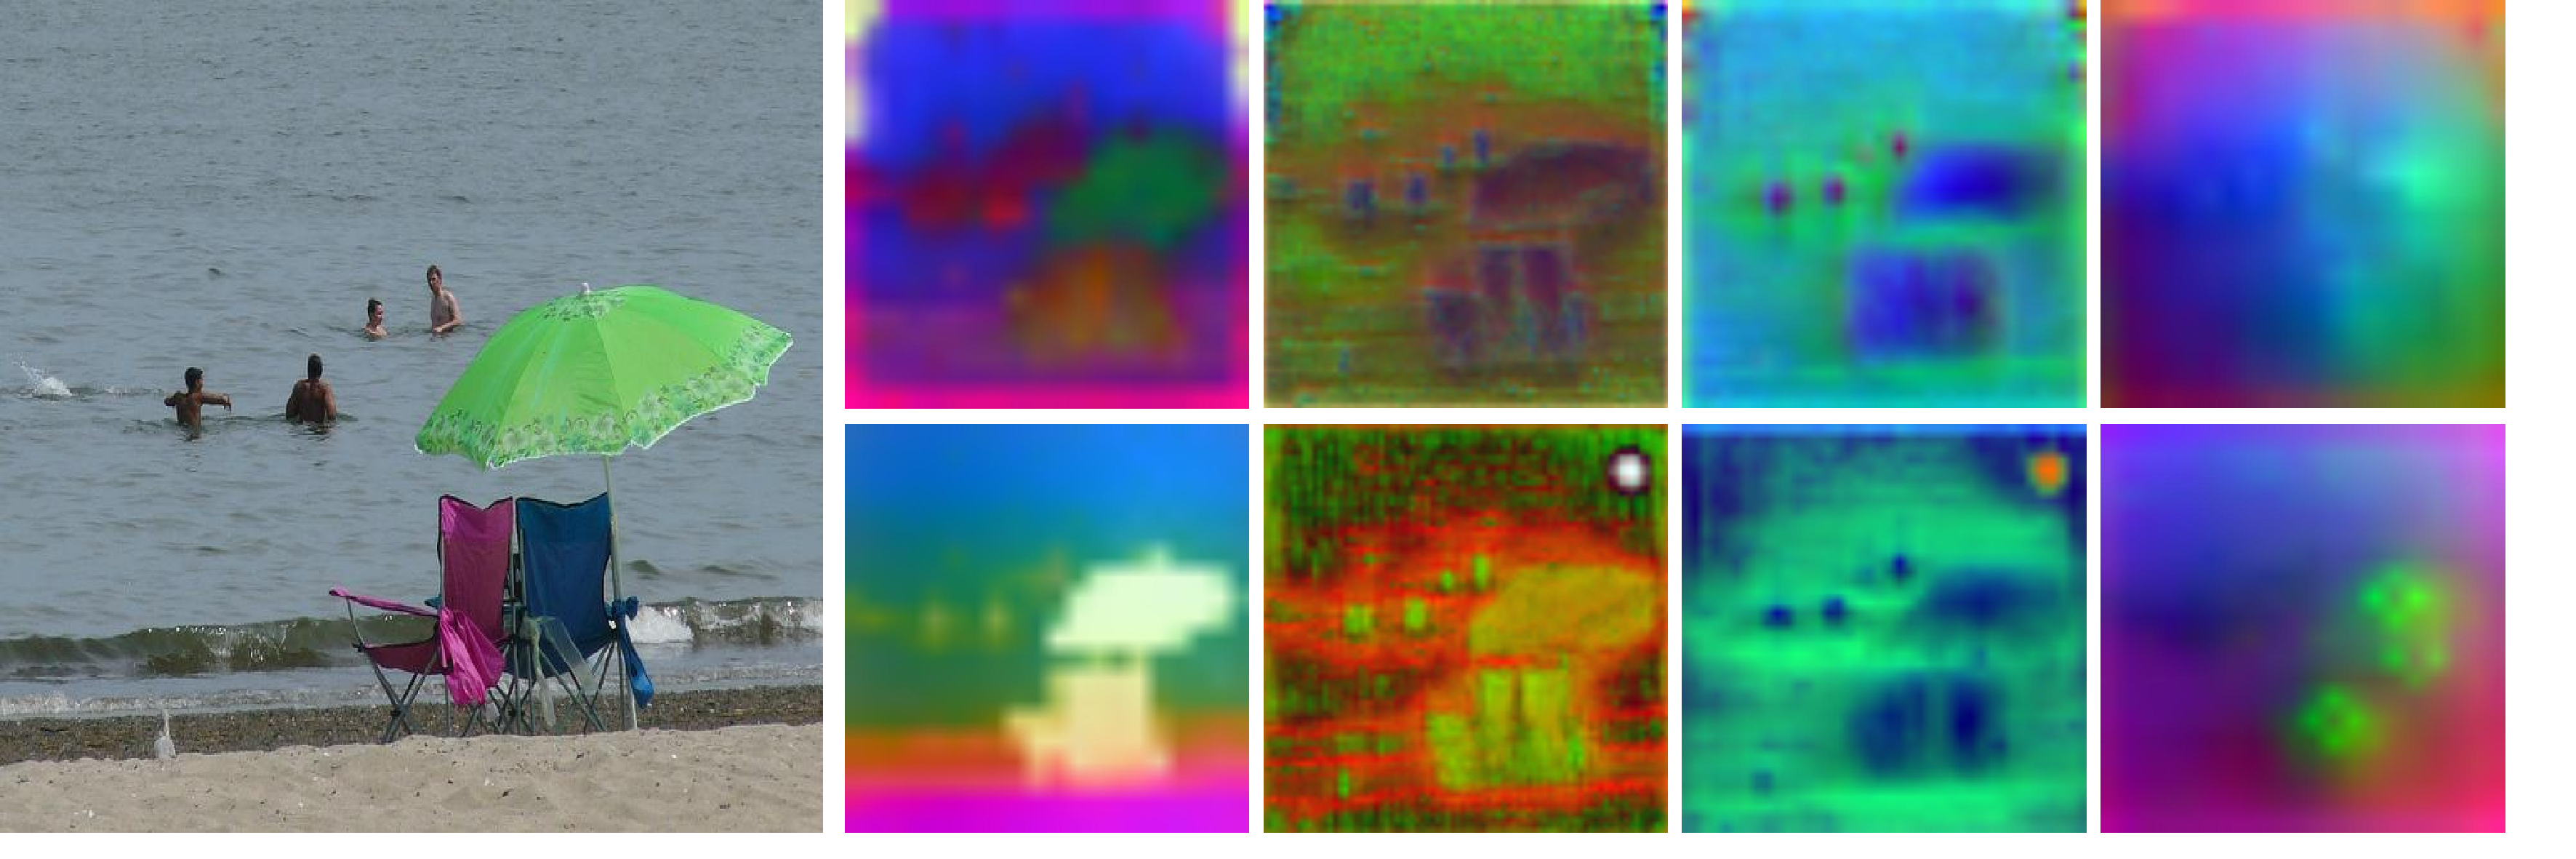
\includegraphics[width=1\linewidth]{figures/feature_map_comparison.pdf}
    \caption{\textbf{Comparison of dense features.} We compare the feature map quality of DEIM-L (top) and \ourmethod-L (bottom) by projecting dense outputs to RGB space using PCA. The visualization reveals that our DSI module substantially enhances the semantic representation of AIFI features, which in turn benefits subsequent CCFF features. From left to right: input image, AIFI feature map $F_5$, and multi-scale CCFF features $P_3$, $P_4$, $P_5$.}
    \label{fig:feature_map_comparison}
\vspace{-5mm}
\end{figure*}

\subsection{Ablation Study}
We conduct a series of ablation experiments to verify the effectiveness of proposed modules. Unless stated otherwise, all ablation experiments are trained for \textbf{36 epochs}. Unspecified hyperparameters or configurations follow the best settings for the corresponding experimental setup.

\begin{table}[!t]
\centering
\caption{\textbf{Results of ablation on DSI and GAM across multiple detectors.} Our method brings consistent and significant gains with zero additional inference cost.}
\label{tab:ablation_main}
\vspace{-2mm}
\resizebox{0.48\textwidth}{!}{
\begin{tabular}{l | ccc}
    \toprule
    Method & AP & AP$_{50}$ & AP$_{75}$ \\
    \midrule
    \textbf{RT-DETRv2-L} & 52.1 & 70.2 & 56.7 \\
    w/ DSI & 52.3 \textcolor{cvprblue}{(+0.2)} & 70.4 \textcolor{cvprblue}{(+0.2)} & 56.4 \textcolor{red}{(-0.3)} \\
    w/ DSI+GAM & \textbf{52.6} \textbf{\textcolor{cvprblue}{(+0.5)}} & \textbf{70.7} \textbf{\textcolor{cvprblue}{(+0.5)}} & \textbf{56.8} \textbf{\textcolor{cvprblue}{(+0.1)}} \\
    \midrule
    \textbf{D-FINE-L} & 53.1 & 70.8 & 57.4 \\
    w/ DSI & 53.2 \textcolor{cvprblue}{(+0.1)} & 70.8 \textcolor{cvprblue}{(+0)} & 57.7 \textcolor{cvprblue}{(+0.3)} \\
    w/ DSI+GAM & \textbf{53.4} \textbf{\textcolor{cvprblue}{(+0.3)}} & \textbf{71.1} \textbf{\textcolor{cvprblue}{(+0.3)}} & \textbf{58.0} \textbf{\textcolor{cvprblue}{(+0.6)}} \\
    \midrule
    \textbf{DEIM-L} & 53.8 & 71.4 & 58.5 \\
    w/ DSI & 53.9 \textcolor{cvprblue}{(+0.1)} & 71.3 \textcolor{red}{(-0.1)} & 58.8 \textcolor{cvprblue}{(+0.3)} \\
    w/ DSI+GAM & \textbf{54.3} \textbf{\textcolor{cvprblue}{(+0.5)}} & \textbf{71.8} \textbf{\textcolor{cvprblue}{(+0.4)}} & \textbf{59.0} \textbf{\textcolor{cvprblue}{(+0.5)}} \\
    \bottomrule
\end{tabular}
}
\vspace{-3mm}
\end{table}

\noindent \textbf{Ablation on DSI and GAM.}
We first assess the effectiveness of DSI and GAM.
As shown in Table~\ref{tab:ablation_main}, applying DSI can bring a slight performance improvement, while further applying GAM can significantly improve the performance gain (0.5 AP), which fully proves the effectiveness of both.
To verify the general applicability of our method, we also conduct experiments on RT-DETRv2 and D-FINE, and the results show that our method can bring consistent performance gains to different detectors.

\begin{table}[!t]
\centering
\caption{\textbf{Results of ablation on semantic injection position.} We compare the effectiveness of applying DSI at different position, corresponding to the strategies in Figure~\ref{fig:module_design}. Aligning only the AIFI output (\(F_5\)) yields the best performance.}
\label{tab:semantic_location}
\resizebox{0.48\textwidth}{!}{
\begin{tabular}{l | ccc c | ccc}
    \toprule
    Position & $S_{3}$ & $S_{4}$ & $S_{5}$ & $F_{5}$ & AP & AP$_{50}$ & AP$_{75}$ \\
    \midrule
    Baseline & - & - & - & - & 53.8 & 71.4 & 58.5 \\
    \hline
    \multirow{4}{*}{Backbone} & \checkmark & - & - & - & 53.7 & 71.2 & 58.4 \\
    & - & \checkmark & - & - & 53.7 & 71.3 & 58.4 \\
    & - & - & \checkmark & - & 53.8 & 71.3 & 58.5 \\
    & \checkmark & \checkmark & \checkmark & - & 53.7 & 71.3 & 58.5 \\
    \hline
    Hybrid & \checkmark & \checkmark & \checkmark & \checkmark & 53.8 & 71.4 & 58.4 \\
    \hline
    AIFI & - & - & - & \checkmark & \textbf{54.3} & \textbf{71.8} & \textbf{59.0} \\
    \bottomrule
\end{tabular}
}
\vspace{-3mm}
\end{table}

\noindent \textbf{Ablation on semantic injection position.}
To validate the choice of injection position, we compare the strategies shown in Figure~\ref{fig:module_design}. Results in Table~\ref{tab:semantic_location} indicate that directly applying semantic supervision to backbone features (\(S_3\), \(S_4\), or \(S_5\)) individually or jointly yields no improvement. Similarly, the hybrid approach (strategy (b)) that aligns both backbone and \(F_5\) features provides no gain (53.8 AP). 

In contrast, our design (strategy (c)), which aligns only the AIFI output \(F_5\), achieves a clear 0.5 AP improvement (54.3 AP). 
This demonstrates that maintaining richer semantics in \(F_5\) is crucial for enhancing detection performance, as it plays a key role in propagating high-level semantic information to subsequent feature hierarchies. Furthermore, the ineffectiveness of the hybrid approach suggests that simultaneously aligning features from the CNN-based backbone and the Transformer-based AIFI may introduce optimization conflicts or semantic misalignment. Our chosen strategy is not only more effective but also more efficient. It avoids the complexity of multiple intermediate projections and interpolations, and the gradient from the single \(F_5\) alignment loss naturally flows back to synergistically update both AIFI and the backbone, achieving consistent enhancement with a single, targeted objective.

\begin{table}[!t]
\centering
\caption{\textbf{Results of ablation on the feature projector.}}
\label{tab:ablation_projector}
\resizebox{0.48\textwidth}{!}{
\begin{tabular}{l | ccc}
    \toprule
    Projector Arch. & AP & AP$_{50}$ & AP$_{75}$ \\
    \hline
    Baseline & 53.8 & 71.4 & 58.5 \\
    \hline
    w/ 1x1 Conv & 53.8 & 71.5 & 58.5 \\
    w/ MLP & 54.2 & 71.7 & 59.0\\
    w/ Linear & \textbf{54.3} \textcolor{cvprblue}{(+0.5)} & \textbf{71.8} \textcolor{cvprblue}{(+0.4)} & \textbf{59.0} \textcolor{cvprblue}{(+0.5)} \\
    \bottomrule
\end{tabular}
}
\end{table}


\begin{table}[!t]
\centering
\caption{\textbf{Results of ablation on the alignment loss.} The cosine similarity loss demonstrates superior performance. DEIM-M is adopted as the baseline. All reported results are obtained from models trained for 90 epochs with 12 epochs EMA following the training protocol of DEIM.}
\label{tab:ablation_loss}
\resizebox{0.48\textwidth}{!}{
\begin{tabular}{l | ccc}
    \toprule
    Loss Function & AP & AP$_{50}$ & AP$_{75}$ \\
    \midrule
    Baseline & 52.5 & 69.9 & 57.2 \\
    \hline
    w/ MSE Loss & 52.7 & 70.0 & 57.4 \\
    w/ Cosine Similarity & \textbf{53.5} \textcolor{cvprblue}{(+1.0)} & \textbf{71.1} \textcolor{cvprblue}{(+1.2)} & \textbf{58.1} \textcolor{cvprblue}{(+0.9)} \\
    \bottomrule
\end{tabular}
}
\end{table}

\begin{table}[htbp]
\centering
\setlength{\tabcolsep}{4.3pt}
\renewcommand{\arraystretch}{1}
\caption{\textbf{Ablation on the loss weighting strategy.} GAM consistently surpasses the best-tuned static weight. DEIM-L is adopted as the baseline. All reported results are obtained from models trained for 50 epochs with 8 epochs EMA following~\cite{huang2025deim}.}
\label{tab:ablation_gam}
\vspace{-5mm}
\begin{tabular}{c|cccccc}
    \multicolumn{7}{l}{}\\
    \toprule
    $\lambda$ & 0.1 & 0.2 & 0.4 & 1 & 2 & 4 \\
    \arrayrulecolor{gray}\midrule
    AP$^{val}$ & 54.7 & 54.7 & 54.8 & 54.9 & \underline{55.0} & \underline{55.0}  \\
    \arrayrulecolor{black}\midrule[0.8pt]
    $\lambda$ & \underline{10} & \textbf{20} & \underline{30} & 50 & 100 & \textbf{GAM}\\
    \arrayrulecolor{gray}\midrule
    AP$^{val}$ & \underline{55.0} & \textbf{55.1} & \underline{55.0} & 54.9 & 54.6 &  \textbf{55.4} \\
    \arrayrulecolor{black}\bottomrule
\end{tabular}
\end{table}

\begin{figure}[!t]
    \centering
    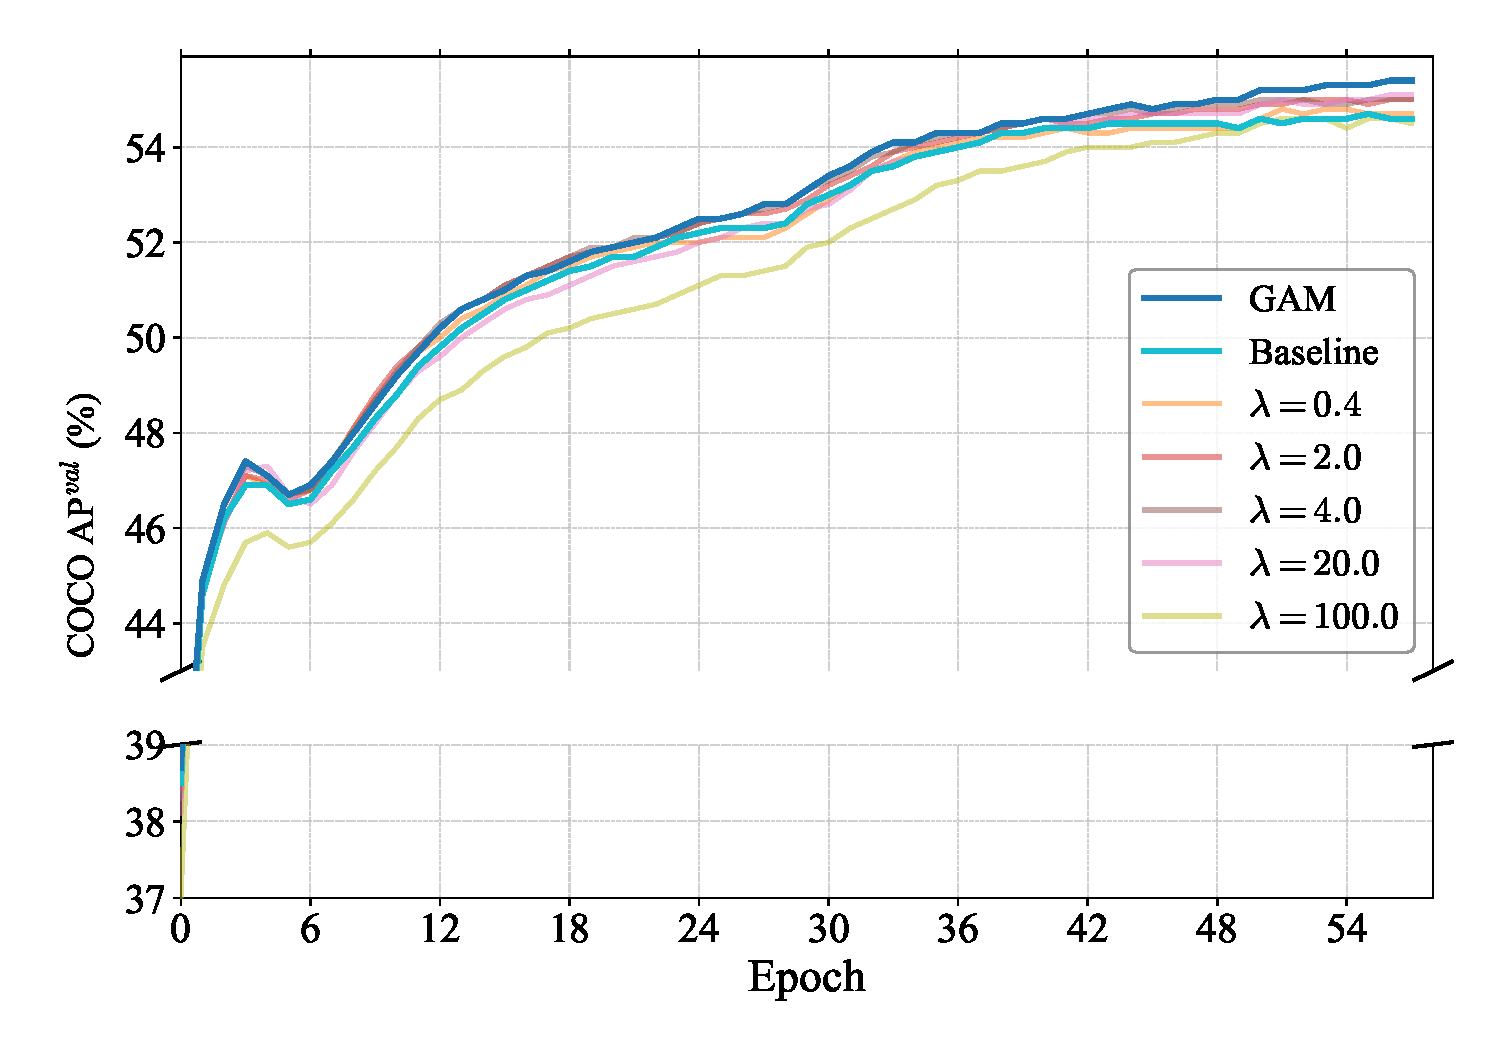
\includegraphics[width=\linewidth]{figures/epoch_vs_ap_broken_axis.pdf}
    \vspace{-5mm}
    \caption{\textbf{Validation AP evolution on COCO during training.} We compare our dynamic GAM with a baseline model and several static $\lambda$ values for the DSI loss. The GAM strategy consistently outperforms all static configurations, showcasing its ability to provide stable and effective supervision throughout the training process.}
    \label{fig:gam_training_curve}
    \vspace{-5mm}
\end{figure}

\noindent \textbf{Design of the feature projector.}
The feature projector is a crucial component for bridging the student and teacher feature spaces. We explore several architectural choices, as detailed in Table~\ref{tab:ablation_projector}. An linear-based projector yields the best results, striking an optimal balance between expressive power and parameter efficiency. 


\noindent \textbf{Choice of loss function.}
We further study the alignment loss of DSI.
We compare the Mean Squared Error (MSE) loss and the Cosine Similarity loss in Table \ref{tab:ablation_loss}, with the latter outperforming the former, validating our hypothesis that aligning feature direction is more crucial.


\noindent \textbf{Comparison of GAM and static weights.}
Finally, we validate the proposed GAM against static weights. The superiority of GAM in navigating the training dynamics is further illustrated in Figure~\ref{fig:gam_training_curve}, which plots the validation AP over epochs. As shown, the curve for GAM consistently remains above the baseline and all static weight configurations, demonstrating a clear and stable performance advantage throughout the training process.

Table~\ref{tab:ablation_gam} details the results for static weight and GAM. For static weighting, performance peaks at $\lambda=20$, achieving 55.1 AP, but degrades with either smaller or larger values. However, observing the training curve in Figure~\ref{fig:gam_training_curve}, we find that even this optimal static weight ($\lambda=20$) leads to slower convergence in the early-to-mid stages, highlighting the inherent limitations of a fixed hyperparameter. Our experiments indicate that GAM achieves the best performance (55.4 AP).

\noindent \textbf{Feature visualization.}
Figure~\ref{fig:feature_map_comparison} visually compares the feature maps between DEIM-L and our RT-DETRv4-L. Notably, our model enriches the semantic content of the AIFI feature $F_5$, leading to more precise and distinguishable object contours and backgrounds across the subsequent multi-scale features $P_3$, $P_4$, and $P_5$. In particular, $P_5$ exhibits a markedly stronger and more concentrated response to object regions.